\chapter{Introdução}

\section{Otimização Combinatória}

Definição: Problema de Otimização

\begin{itemize}
    \item Entrada (instância)
    \item Conjunto de soluções viáveis
          \begin{itemize}
              \item Soluções válidas
              \item Respeitam as restrições do problema
          \end{itemize}
\end{itemize}

Quero achar a melhor solução

\begin{itemize}
    \item Função objetivo
          \begin{itemize}
              \item Asssocia um valor real a cada solução viável
          \end{itemize}
\end{itemize}

Melhor: maximização ou minimização -- De acordo com a função objetivo

Otimização Combinatória

\begin{itemize}
    \item Variáveis discretas
    \item O conjunto de soluções viáveis é finito
\end{itemize}

\begin{example}
    Problema do escalonamento

    Dadas $n$ tarefas, cada uma com uma duração, alocá-las em $m$ máquinas minimizando a maior soma de tempos (\textit{makespan}).

    \vspace{\baselineskip}
    Instâncias

    \qquad $m = 2$
    \begin{center}
        \begin{tikzpicture}[tempo/.style 2 args={rectangle split,
                        rectangle split horizontal, draw=#2, rectangle split parts=#1, fill=#2!20, outer sep=1mm}]
            \node[tempo={3}{blue}, label=below:$t_1$] (t1) at (0, 0) {};
            \node[tempo={2}{red}, label=below:$t_2$] (t2) [right=of t1] {};
            \node[tempo={2}{green}, label=below:$t_3$] (t3) [right=of t2] {};
            \node[tempo={4}{orange}, label=below:$t_4$] (t4) [right=of t3] {};
        \end{tikzpicture}
    \end{center}

    Exemplos de soluções

    \begin{multicols}{2}
        \begin{tabular}{l|l}
            $M_1$ & \tikzmark{1m11} \\
            $M_2$ & \tikzmark{1m21} \\
        \end{tabular}

        \begin{tikzpicture}[remember picture, tempo/.style 2 args={rectangle split, rectangle split horizontal, overlay, draw=#2, rectangle split parts=#1, fill=#2!20, anchor=west}, node distance=1pt]
            \node[tempo={3}{blue}] (t1) at (pic cs:1m11) {};
            \node[tempo={4}{orange}] (t4) [right=of t1] {};
            \node[tempo={2}{red}] (t2) at (pic cs:1m21) {};
            \node[tempo={2}{green}] (t3) [right=of t2] {};
        \end{tikzpicture}

        \begin{center}
            \textit{makespan} = $7$
        \end{center}

        \columnbreak

        \begin{tabular}{l|l}
            $M_1$ & \tikzmark{1m12} \\
            $M_2$ & \tikzmark{1m22} \\
        \end{tabular}

        \begin{tikzpicture}[remember picture, tempo/.style 2 args={rectangle split, rectangle split horizontal, overlay, draw=#2, rectangle split parts=#1, fill=#2!20, anchor=west}, node distance=1pt]
            \node[tempo={3}{blue}] (t1) at (pic cs:1m12) {};
            \node[tempo={2}{red}] (t2) [right=of t1] {};
            \node[tempo={4}{orange}] (t4) at (pic cs:1m22) {};
            \node[tempo={2}{green}] (t3) [right=of t4] {};
        \end{tikzpicture}

        \begin{center}
            \textit{makespan} = 6
        \end{center}
    \end{multicols}
\end{example}

\section{Definições básicas}

\subsection{Grafos}

Estrutura matemática que representa relacionamentos par-a-par (arestas) entre objetos (vértices).

Formalização: $G = (V, E)$

\qquad $V =$ conjunto de vértices

\qquad $E =$ conjunto de arestas

$E$ é um conjunto de pares.

\begin{example}
    \begin{multicols}{2}
        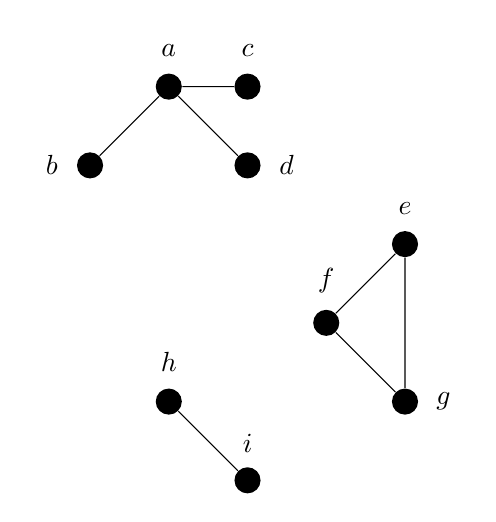
\begin{tikzpicture}[every node/.style={circle, fill}]
            \node[label=$a$] (a) at (0, 0) {};
            \node[label=left:$b$] (b) at (-1, -1) {};
            \node[label=$c$] (c) at (1, 0) {};
            \node[label=right:$d$] (d) at (1, -1) {};
            \draw (a) -- (b) (a) -- (c) (a) -- (d);

            \node[label=$e$] (e) at (3, -2) {};
            \node[label=$f$] (f) at (2, -3) {};
            \node[label=right:$g$] (g) at (3, -4) {};
            \draw (e) -- (f) -- (g) -- (e);

            \node[label=$h$] (h) at (0, -4) {};
            \node[label=$i$] (i) at (1, -5) {};
            \draw (h) -- (i);
        \end{tikzpicture}

        \columnbreak

        $V = \{a, b, c, d, e, f, g, h, i\}$

        $E = \{(a, b), (a, c), (a, d), (h, i), \dots\}$
    \end{multicols}
\end{example}

Tipos comuns de grafos

\begin{itemize}
    \item Caminho
          \begin{itemize}
              \item Conexo
              \item Não possui bifurcação
          \end{itemize}
          \begin{example}
              \begin{center}
                  \tikz[every node/.style={circle, fill}]
                  \draw (0, 0) node {} -- (1, 0) node {} -- (2, 0) node {} -- (3, 1) node {} -- (4, 0) node {} -- (4, -1) node {} -- (5, 0) node {};
              \end{center}
          \end{example}
    \item Circuito
          \begin{itemize}
              \item Fecha o ciclo
          \end{itemize}
          \begin{example}
              \begin{center}
                  \tikz[every node/.style={circle, fill}]
                  \draw (0, 0) node(a) {} -- (1, 1) node {} -- (2, 1) node {} -- (3, 0) node {} -- (3, -1) node {} -- (2, -2) node {} -- (1, -1) node {} -- (a);
              \end{center}
          \end{example}
    \item Completo
          \begin{itemize}
              \item Todos os nós conectados entre si
              \item Representado por $K_n$, sendo $n$ o número de vértices
          \end{itemize}
          \begin{example}
              \begin{center}
                  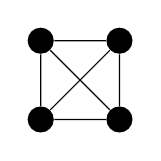
\begin{tikzpicture}[every node/.style={circle, fill}]
                      \node (a) at (0, 0) {};
                      \node (b) at (1, 0) {};
                      \node (c) at (0, 1) {};
                      \node (d) at (1, 1) {};

                      \draw (a) -- (b) (a) -- (c) (a) -- (d);
                      \draw (b) -- (c) (b) -- (d) -- (c);
                  \end{tikzpicture}
              \end{center}
          \end{example}
    \item Bipartidos
          \begin{itemize}
              \item Dois subconjuntos de vértices sem arestas entre split
              \item Tipos de entidades distintas
          \end{itemize}
          \begin{example}
              \begin{center}
                  \begin{tikzpicture}[n/.style={circle, fill}]
                      \node[n] (a) at (0, 0) {};
                      \node[n] (b) at (0, 1) {};
                      \node[n] (c) at (0, 2) {};
                      \node[n] (d) at (0, 3) {};

                      \node[n] (e) at (2, 0) {};
                      \node[n] (f) at (2, 1) {};
                      \node[n] (g) at (2, 2) {};

                      \node[draw, ellipse, fit=(a)(b)(c)(d)] {};
                      \node[draw, ellipse, fit=(e)(f)(g)] {};

                      \draw (a) -- (e) -- (c) (a) -- (f) (d) -- (g);
                  \end{tikzpicture}
              \end{center}
          \end{example}
    \item Árvores
          \begin{itemize}
              \item Grafos conexos e acíclicos
              \item Caminhos são um tipo específico de árvore
              \item Para qualquer par de nós $a$ e $b$, existe um único caminho conectando $a$ a $b$
          \end{itemize}
          \begin{example}
              \begin{center}
                  \tikz[every node/.style={circle, fill}]
                  \draw (0, 0) node {} -- (1, 0) node (a) {} -- (2, 1) node {} (a) -- (2, -1) node {} -- (3, 0) node (b) {} -- (4, 1) node {} (b) -- (4, 0) node {} (b) -- (4, -1) node {};
              \end{center}
          \end{example}
\end{itemize}

Os grafos podem ser \underline{orientados} (ou dirigidos) ou \underline{não-orientados}. No caso dos grafos orientados, as arestas (também chamadas de arcos) têm uma direção.

Os grafos também podem ter pesos (ou custos) associados às arestas.

\begin{example}
    \begin{center}
        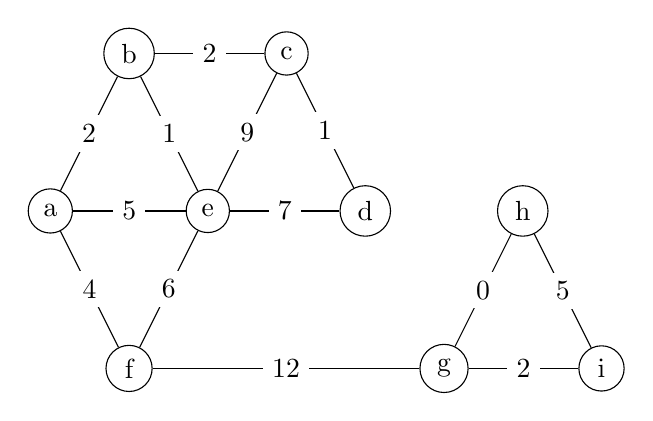
\begin{tikzpicture}[every node/.style={fill=white}, n/.style={circle, draw}]
            \node[n] (a) at (0, 0) {a};
            \node[n] (b) at (1, 2) {b};
            \node[n] (c) at (3, 2) {c};
            \node[n] (d) at (4, 0) {d};
            \node[n] (e) at (2, 0) {e};
            \node[n] (f) at (1, -2) {f};
            \node[n] (g) at (5, -2) {g};
            \node[n] (h) at (6, 0) {h};
            \node[n] (i) at (7, -2) {i};

            \draw (a) edge node {2} (b) edge node {5} (e) edge node {4} (f)
            (b) edge node {2} (c) edge node {1} (e)
            (c) edge node {1} (d) edge node {9} (e)
            (d) edge node {7} (e)
            (e) edge node {6} (f)
            (f) edge node {12} (g)
            (g) edge node {0} (h) edge node {2} (i)
            (h) edge node {5} (i);
        \end{tikzpicture}
    \end{center}
\end{example}

Os pesos são formalizados como uma função separada: $f: E \mapsto \mathbb{R}$.

\subsection{Análise de algoritmos}

Mostra que

\begin{itemize}
    \item Um algoritmo está correto
    \item Estimar o tempo de execução
\end{itemize}

É uma análise matemática, então \underline{não é preciso implementar o algoritmo}.

Notação assintótica: termos de menor ordem e constantes são de desconsiderados.

$20n^2 + 500n \rightarrow O(n^2)$

\section{Exemplos de problemas}

\subsection{Árvore de Steiner}

\begin{itemize}
    \item \textbf{Entrada:} $G = (V, E)$ com $V = R \cup S$, sendo $R$ terminais e $S$ vértices de Steiner, e função $w$ de peso na arestas.
    \item \textbf{Soluções viáveis:} árvores que conectam todos os vértices em $R$.
    \item \textbf{Função objetivo:} soma dos pesos das arestas na árvore.
    \item \textbf{Objetivo:} enconctrar uma árvore de peso mínimo.
\end{itemize}

\subsection{\textit{Bin Packing}/Empacotamento}

\begin{itemize}
    \item \textbf{Entrada:} conjunto $L = \{1,\dots,n\}$ de itens retangulares, item $i$ com largura $w_i$ e altura $h_i$, largura $W$ e altura $H$ do recipiente retangular.
    \item \textbf{Soluções viáveis:} partição $L_1, L_2, \dots, L_q$ de $L$ tal que os itens em $L_k$ cabem num recipiente $W \times H$.
    \item \textbf{Função objetivo:} número $q$ de recipientes (\textit{bins}) utilizados.
    \item \textbf{Objetivo:} encontrar solução de custo mínimo.
\end{itemize}

\subsection{Caixeiro Viajante (TSP - \textit{Traveling Salesman Problem})}

\begin{itemize}
    \item \textbf{Entrada:} $G = (V, E)$ e função $w$ de peso nas arestas.
    \item \textbf{Soluções viáveis:} circuitos hamiltonianos (passam por todos os vértices sem repetição) de $G$.
    \item \textbf{Função objetivo:} soma dos pesos das arestas do circuito.
    \item \textbf{Objetivo:} encontrar o circuito de menor custo
\end{itemize}

\subsection{Problema da Mochila}

\begin{itemize}
    \item \textbf{Entrada:} conjunto de $n$ itens, cada item $i$ tem peso $w_i$ e valor $v_i$ e tamanho $W$ da mochila.
    \item \textbf{Soluções viáveis:} conjuntos de itens $S \subseteq \{1,\dots,n\}$ com $\sum_{i \in S} w_i \leq W$.
    \item \textbf{Função objetivo:} soma dos valores dos itens em $S$.
    \item \textbf{Obejtivo:} encontrar uma solução de valor máximo.
\end{itemize}

\section{Dificuldades}

Primeira abordarem de resolução de problemas: busca por força bruta.

O espaço de busca é finito, então dá para enumerar todas as soluções guardando a melhor encontrada. \underline{Com tempo suficiente}, resolve o problema.

Mas não explora as estruturas combinatórias do problema. $\to$ Muito esforço.

Com um espaço muito grande, fica inviável usar.

\begin{example}
    No TSP qualquer sequência dos $n$ vértices é candidata a solução.

    \vspace{\baselineskip}
    Algoritmo:
    \begin{enumerate}
        \item Gere as $n!$ sequências de vértices
        \item Cada sequência é um circuito hamiltoniano
        \item Calcule seu custo e compare com o melhor já encontrado
    \end{enumerate}

    \textbf{São $\mathbf{(n-1)!}$ sequências no espaço de busca.}
\end{example}

\begin{example}
    No problema da mochila, qualquer subconjunto dos $n$ elementos é candidato a solução.

    \vspace{\baselineskip}
    Algoritmo:
    \begin{enumerate}
        \item Gere os $2^{n}$ possíveis subconjuntos
        \item Para cada um, teste se os itens cabem na mochila $\to$ \underline{Viabilidade}
        \item Se couberem, calcule o custo da soluçào e compare com o melhor já encontrado
    \end{enumerate}

    \textbf{Crescimento exponencial}
\end{example}

\subsection{Complexidade}

\begin{itemize}
    \item Algoritmo eficiente: complexidade de tempo no pior caso é polinomial no tamanho $n$ da entrada $\to O(n^{k})$ com $k$ constante.
    \item Problemas de decisão: Problemas com resposta \underline{sim} ou \underline{não}.
\end{itemize}

Classes de problemas:

\begin{itemize}
    \item \textbf{Classe P:} problemas de decisão que possuem algoritmos eficientes.
    \item \textbf{Classe NP:} problemas de decisão cuja solução ("resposta \underline{sim}") pode ser \underline{verificada} em tempo polinomial.
    \item \textbf{Classe NP-Completo}: problemas Q tais que $\mathrm{Q} \in \mathrm{NP}$ e todo problema \underline{em NP} é redutível a Q.
\end{itemize}

\textbf{Redução}

Um problema A é redutível a B se podemos utilizar um algoritmo que resolve B para resolver A, ou seja, \underline{B é pelo menos tão difícil quanto A}.

Não há um certificado de dificuldade absoluto: "esse problema não é possíel de resolver". Existe a dificuldade relativa: "esse problema é tão complexo quanto aquele".

\begin{itemize}
    \item \textbf{Classe NP-Difícil}: problemas Q tais que todo problema em NP é redutível a Q. Esses problemas não precisam ser necessariamente NP ($\neq$ NP-Completo).
\end{itemize}

\subsection{Abordagens}

Se $\mathrm{P} \neq \mathrm{NP}$, não é possível ter algoritmos para problemas NP-Difíceis que:
\begin{itemize}
    \item Encontrem soluções ótimas
    \item Em tempo polinomial
    \item Para qualquer entrada
\end{itemize}

Tem que abrir mão de alguma característica

\begin{itemize}
    \item Métodos exatos
          \begin{itemize}
              \item Não funcionam em tempo hábil (exponencial ou superpolinomial)
              \item Ao contrário da força bruta, explora as estruturas combinatórias para eliminar pedaços do espaço de busca para facilitar
          \end{itemize}
    \item Heurísticas
          \begin{itemize}
              \item Não encontra necessariamente soluções ótimas
              \item Procura soluções ``boas o bastante''
              \item Avaliação empírica com o uso de \textit{benchmarks} de instâncias
          \end{itemize}
    \item Algoritmos de aproximação
          \begin{itemize}
              \item Não encontra necessariamente soluções ótimas (subconjunto das heurísticas)
              \item Garantia de que o algoritmo é polinomial
              \item Garantia de que o resultado vai estar dentro de uma margem de erro da solução ótima
          \end{itemize}
    \item Parametrização
          \begin{itemize}
              \item Não funciona para todas as instâncias
              \item Um parâmetro é fixado
              \item Garantia de encontrar a solução ótima para as instâncias com o parâmetro fixo
          \end{itemize}
\end{itemize}

\section{Métodos exatos}

\begin{itemize}
    \item Procuram a solução ótima
    \item Considera as estruturas combinatórias do problema $\to$ Diferença da força bruta
    \item Não garante tempo polinomial no pior caso (Problemas NP-Difíceis)
\end{itemize}

Exemplos de métodos exatos

\begin{itemize}
    \item Algoritmos gulosos
    \item Programação dinâmica
    \item \textbf{\textit{Branch and bound}}
    \item \textbf{Programação linear / Programação linear inteira}
    \item Programação por restrições $\times$
\end{itemize}

\subsection{Algoritmos gulosos}

Realizam decisões melhores em curto prazo, esperando que isso leve ao resultado ótimo.

Existem casos que um algoritmo guloso resolve o problema em tempo polinomial para todas as instâncias. Exemplos:

\begin{itemize}
    \item Caminho mínimo $\to$ Dijkstra
    \item MST $\to$ Prim e Kruskal
    \item Compressão de Dados $\to$ Huffman
    \item Mochila Fracionária
\end{itemize}

Para problemas NP-Difíceis, dá para usar algoritmos gulosos \underline{como heurísticas}.

\subsubsection{Mochila Fracionária}

Os itens que são colocados na mochila podem ser divisíveis. Pode pegar frações de itens.

Objetivo: pegar os itens com o maior custo-benefício. Razão $\frac{\mathrm{valor}}{\mathrm{peso}}$. Garantir que ninguém melhor está fora da mochila.

\begin{example}
    \begin{multicols}{2}

        $W = 50$

        $v_1 = 60$ \hspace{10pt} $w_1 = 10$ \hspace{10pt} $\frac{v_1}{w_1} = 6$

        $v_2 = 100$ \hspace{10pt} $w_2 = 20$ \hspace{10pt} $\frac{v_2}{w_2} = 5$

        $v_3 = 120$ \hspace{10pt} $w_3 = 30$ \hspace{10pt} $\frac{v_3}{w_3} = 4$

        \columnbreak

        Ordem decrescente: 1, 2, 3

        Fração item 1: $100\%$

        Espaço livre: $50 - 10 = 40$

        Fração item 2: $100\%$

        Espaço livre: $40 - 20 = 20$

        Fração item 3: $\frac{20}{30} = 66\%$

        Espaço livre: $20 - 20 = 0$
    \end{multicols}
\end{example}

\begin{algorithm}
    \SetAlgoLined
    \SetKwFunction{MochilaFrac}{MochilaFrac}

    \Fn{\MochilaFrac{$n: \mathrm{itens}$, $w: \mathrm{peso}$, $v: \mathrm{valor}$, $W: \mathrm{capacidade}$}}{

        Ordene e renomeie os itens para que $\frac{v_1}{w_1} \geq \frac{v_2}{w_2} \geq \cdots \geq \frac{v_n}{w_n}$\;

        Seja $q$ um inteiro tal que $X = \sum_{i=1}^{q}w_i \leq W$ e $\sum_{i=1}^{q+1} w_i > W$

        Cabe ainda uma fração $\frac{W-X}{w_{q+1}}$ do item $q + 1$

        \Retorna{$v_1 + v_2 + \dots + v_q + v_{q+1} \frac{W-X}{w_{q+1}}$}
    }
\end{algorithm}

\subsection{\textit{Branch and Bound}}

Busca exaustiva inteligente: enumeração (\textit{branch}) e poda (\textit{bound}).

Cria uma árvore de enumeração das soluções e, elimina ramos pouco promissores (não percorre esses ramos).

\begin{itemize}
    \item Como fazer a enumeração?
    \item Como percorrer a árvore?
    \item Como podar?
\end{itemize}

\subsubsection{Caixeiro Viajante}

Enumerar todas as sequências de vértices sendo que

\begin{itemize}
    \item Cada nó da árvore representa um nó do grafo original
    \item Cada ramificação na árvore representa uma aresta percorrida
\end{itemize}

\begin{example}
    \centering
    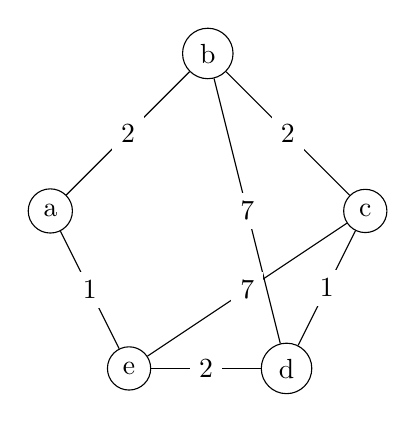
\begin{tikzpicture}[every node/.style={fill=white}, n/.style={circle, draw}]
        \node[n] (a) at (0, 0) {a};
        \node[n] (b) at (2, 2) {b};
        \node[n] (c) at (4, 0) {c};
        \node[n] (d) at (3, -2) {d};
        \node[n] (e) at (1, -2) {e};

        \draw (a) edge node {2} (b);
        \draw (a) edge node {1} (e);
        \draw (b) edge node {2} (c);
        \draw (b) edge node {7} (d);
        \draw (c) edge node {1} (d);
        \draw (c) edge node {7} (e);
        \draw (d) edge node {2} (e);
    \end{tikzpicture}
\end{example}

Árvore de enumeração:

\begin{example}
    \centering
    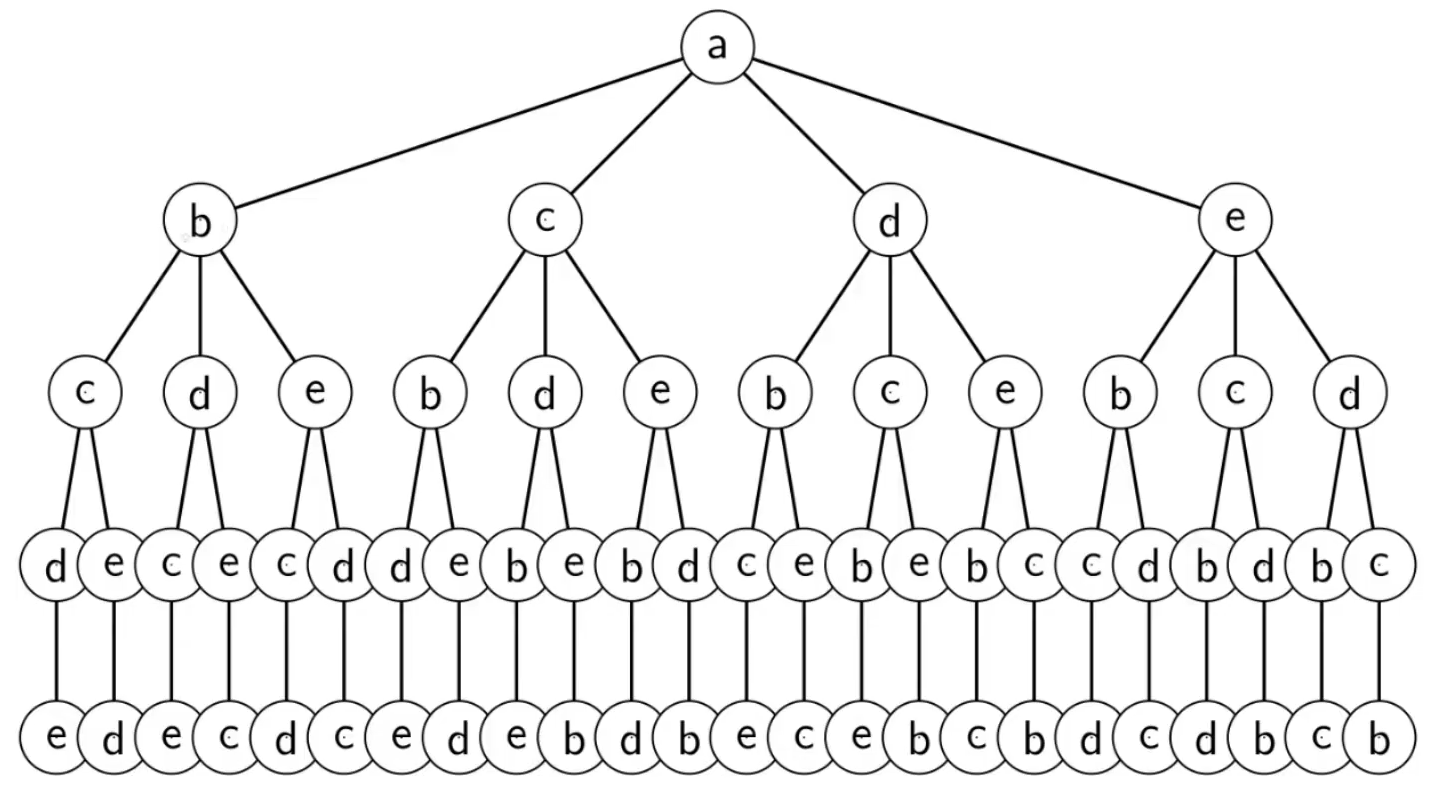
\includegraphics[width=.95\linewidth]{img/arvore_enumeracao_tsp.png}
\end{example}

Pode podar aqueles ramos que indicam um caminho impossível (sem aresta)

\begin{example}
    \centering
    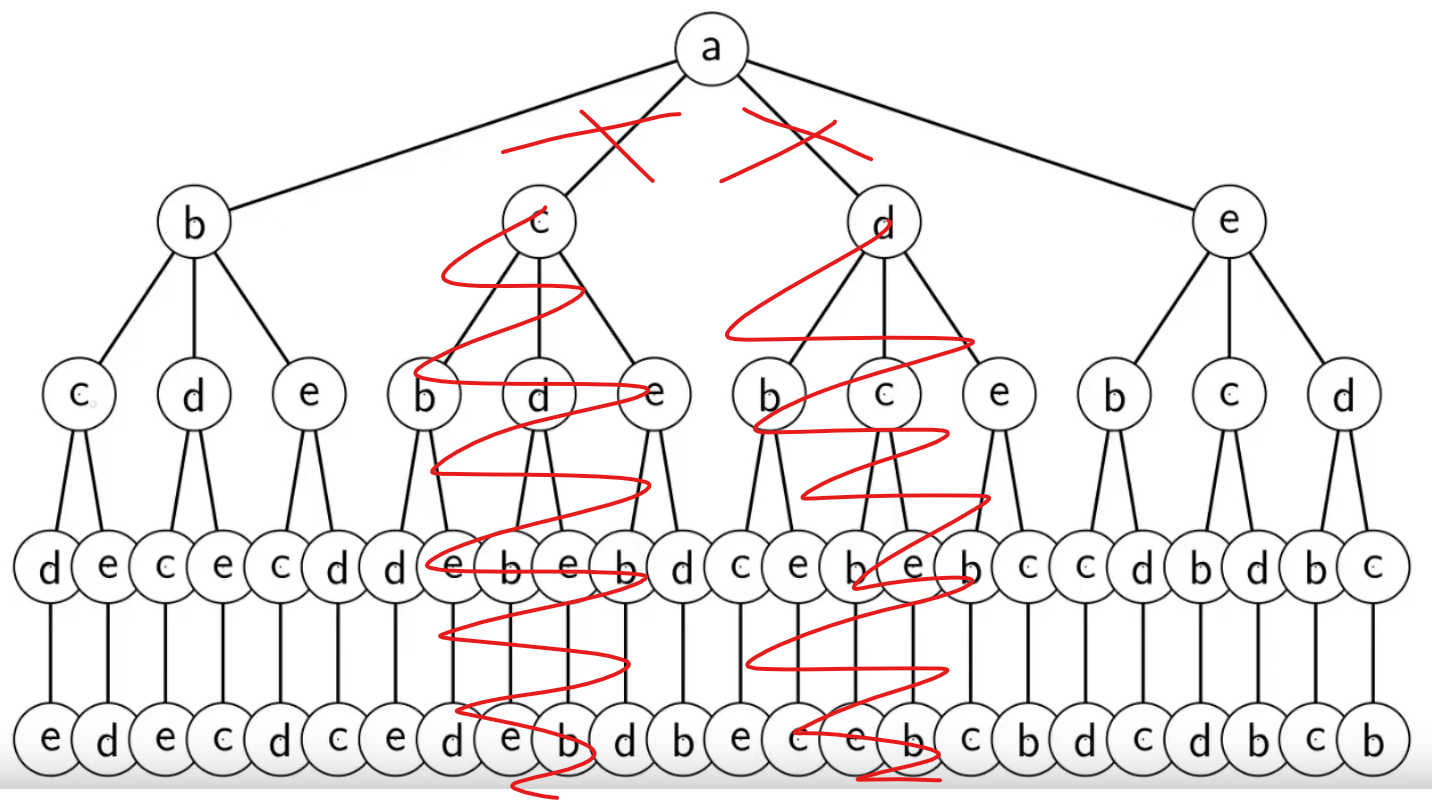
\includegraphics[width=.95\linewidth]{img/arvore_podada_tsp.png}
\end{example}

Mais podas podem ser feitas

\begin{example}
    \centering
    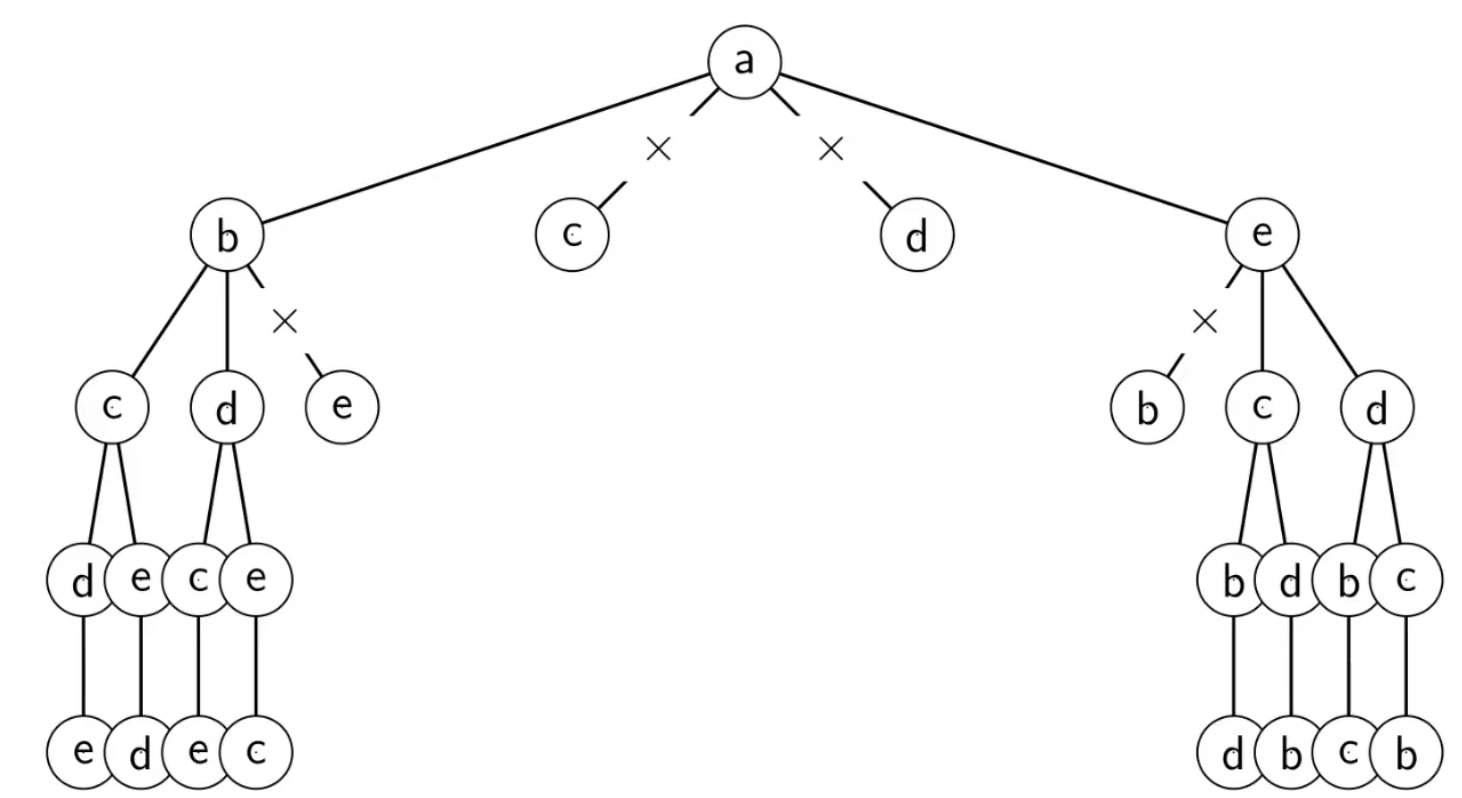
\includegraphics[width=.95\linewidth]{img/arvore_podada_tsp_2.png}
\end{example}

Levando os custos das arestas em consideração:

O caminho $a \xrightarrow{2} b \xrightarrow{2} c \xrightarrow{1} d \xrightarrow{2} e \xrightarrow{1} a$ tem custo total $8$.

O caminho $a \xrightarrow{2} b \xrightarrow{7} d$ tem custo $9$ por si só. Então tudo abaixo vai ser pior que o caminho anterior, não é promissor usar.

Com todos esses caminhos removidos, a árvore final que precisa ser percorrida fica:

\begin{example}
    \centering
    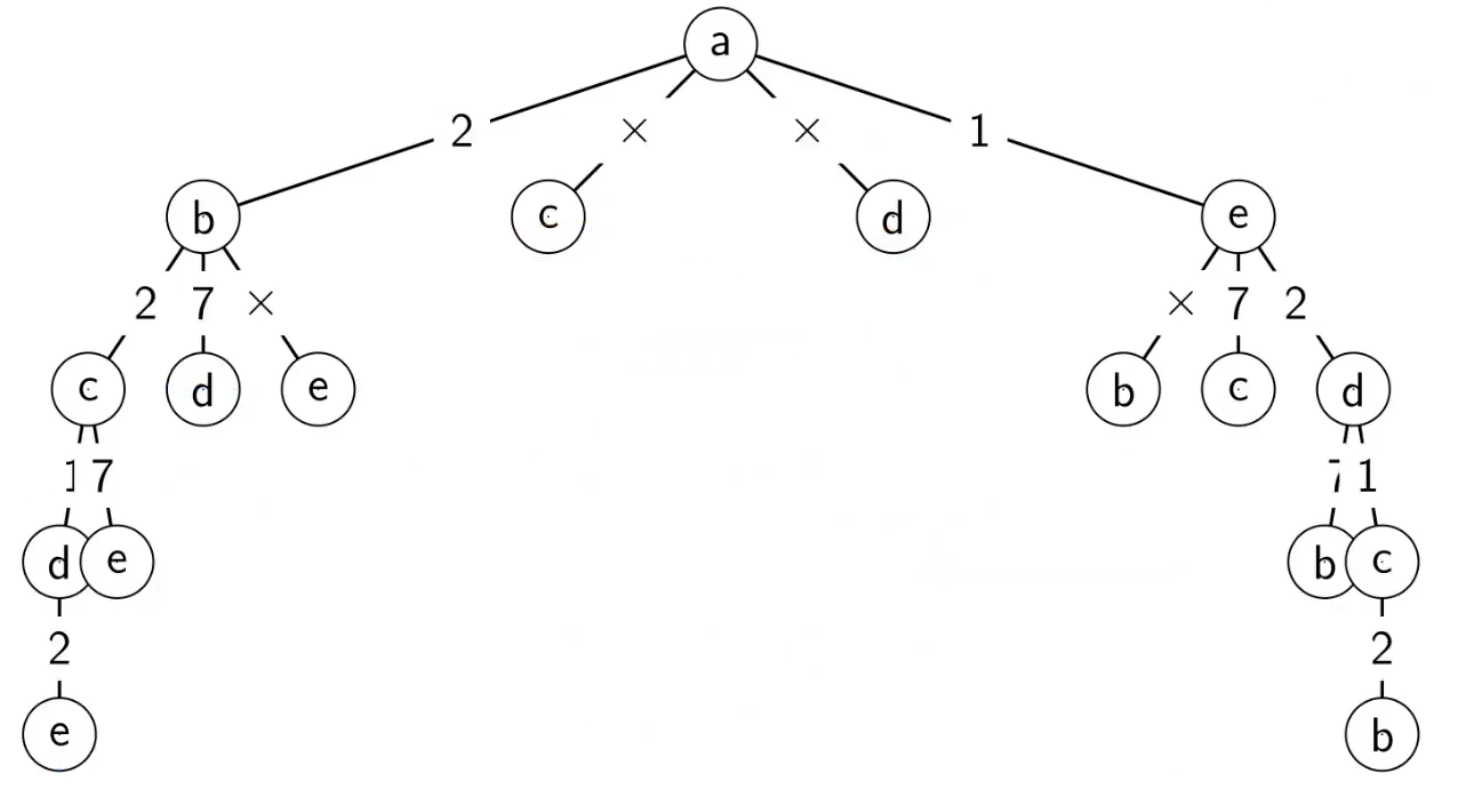
\includegraphics[width=.95\linewidth]{img/arvore_podada_tsp_final.png}
\end{example}

\subsection{Programação linear (inteira)}

Modelo matemático de otimização.

\begin{itemize}
    \item Conjunto variáveis relacionamentos
    \item Conjunto de restrições $\to$ inequações lineares
    \item Função objetivo $\to$ expressão linear
\end{itemize}

Sempre trabalhar com constantes multiplicando variáveis e soma deses valores.

Uma solução é viável se todas as restrições são atendidas.

\vspace{\baselineskip}

A forma padrão para um problema de \underline{minimização} com $n$ variáveis e $m$ restrições é:

\vspace{\baselineskip}

\begin{center}
    minimizar $\sum_{j=1}^{n}c_jx_j$

    sujeito a $\sum_{j=1}^{n}a_{ij}x_j \geq b_i \forall i \in \{1,\dots,m\}$

    $x_j \geq 0 \forall j \in \{1,\dots,n\}$
\end{center}

$a_{ij}$, $b_i$ e $c_j$ são constantes.

$x_j$ são variáveis.

Em um programa linear inteiro, as \underline{variáveis são inteiras}.

\subsubsection{Problema da Mochila}

Sejam $x_i$ variáveis binárias que indicam se o item $i$ foi ecolhido.

\begin{center}
    maximizar $\sum_{i=1}^{n}v_ix_i$

    sujeito a $\sum_{i=1}^{n}w_ix_i \leq W$

    $x_i \in \left\{ 0, 1\right\} \forall i \in \left\{ 1, \dots, n\right\}$
\end{center}

\vspace{\baselineskip}

Programas lineares podem ser resolvidos em tempo polinomial $\to$ Mochila fracionária.

Programas lineares \underline{inteiros} são, normalmente, NP-Difíceis.

Resolvedores de PLI usam o \textit{branch and bound} junto com PL.

Roda PL dentro de cada nó para encontrar limitantes inferiores para aquele ramo inteiro. Depois faz a poda.

\section{Heurísticas}

Algoritmos que encontram uma solução viável.

\textbf{Não} garante que seja solução ótima.

Tendem a ser mais rápidos.

Duas categorias:

\begin{itemize}
    \item Construtivas: Constroem uma solução viável
    \item Busca local: Partem de uma solução inicial e tentam melhorar através de modificações
\end{itemize}

\subsection{Heurística construtiva para a Mochila}

\begin{algorithm}
    \SetAlgoLined
    \SetKwFunction{Mochila}{MochilaGuloso}

    \Fn{\Mochila{$n: \mathrm{itens}$, $w: \mathrm{peso}$, $v: \mathrm{valor}$, $W: \mathrm{capacidade}$}}{
        ordene e renomeie os itens para que $\frac{v1}{w_1}\geq\frac{v_2}{w_2}\geq\dots\geq\frac{v_n}{w_n}$\;
        seja $q$ um inteiro tal que $\sum_{i=1}^{q}w_i\leq W$ e $\sum_{i=1}^{q+1} > W$\;
        \Retorna{$v_1+v_2+\dots+v_q$}
    }
\end{algorithm}

Exemplo que não funciona:

\begin{example}
    \begin{multicols}{2}
        $W=B$

        $v_1 = 2$ \quad $w_1 = 1$ \quad $\frac{v_1}{w_1}=2$

        $v_2 = B$ \quad $w_2 = B$ \quad $\frac{v_2}{w_2}=1$

        \columnbreak

        Ordem decrescetnte: 1, 2

        Fração item 1: $100\%$

        Espaço livre: $B - 1$

        Fração item 2: $0\%$
    \end{multicols}
\end{example}

A solução final é fica com valor 1 e espaço livre $B-1$. Mas a solução ótima é, claramente, pegar o item 2. Então a solução gulosa não é ótima, mas é uma solução viável.

\subsubsection{Heurística de busca local para o TSP}

Vizinhança de 2-OPT (troca de 2 arestas) de um circuito hamiltoniano $C$:

\begin{itemize}
    \item Conjunto de circuitos hamiltonianos que são obtidos removendo 2 arestas de $C$ e inserindo outras 2 arestas
\end{itemize}

Exemplo de troca 2-OPT:

\begin{example}
    \centering
    \begin{multicols}{3}
        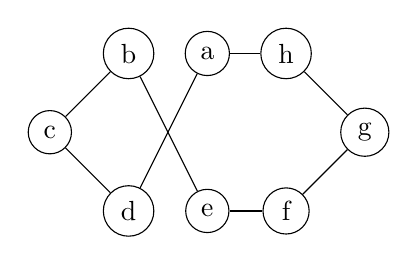
\begin{tikzpicture}[every node/.style={fill=white}, n/.style={circle, draw}]
            \node[n] (c) at (0, 0) {c};
            \node[n] (b) at (1, 1) {b};
            \node[n] (d) at (1, -1) {d};
            \node[n] (a) at (2, 1) {a};
            \node[n] (e) at (2, -1) {e};
            \node[n] (h) at (3, 1) {h};
            \node[n] (f) at (3, -1) {f};
            \node[n] (g) at (4, 0) {g};

            \draw (c) edge (b);
            \draw (b) edge (e);
            \draw (e) edge (f);
            \draw (f) edge (g);
            \draw (g) edge (h);
            \draw (h) edge (a);
            \draw (a) edge (d);
            \draw (d) edge (c);
        \end{tikzpicture}
        \columnbreak
        \vspace*{.8cm}
        {\Huge $\Rightarrow$}
        \columnbreak
        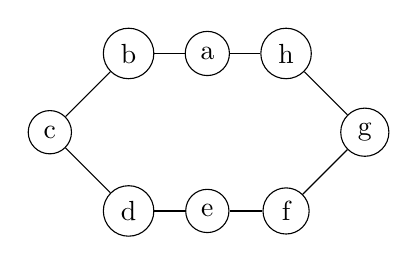
\begin{tikzpicture}[every node/.style={fill=white}, n/.style={circle, draw}]
            \node[n] (c) at (0, 0) {c};
            \node[n] (b) at (1, 1) {b};
            \node[n] (d) at (1, -1) {d};
            \node[n] (a) at (2, 1) {a};
            \node[n] (e) at (2, -1) {e};
            \node[n] (h) at (3, 1) {h};
            \node[n] (f) at (3, -1) {f};
            \node[n] (g) at (4, 0) {g};

            \draw (c) edge (b);
            \draw (b) edge (a);
            \draw (e) edge (f);
            \draw (f) edge (g);
            \draw (g) edge (h);
            \draw (h) edge (a);
            \draw (e) edge (d);
            \draw (d) edge (c);
        \end{tikzpicture}
    \end{multicols}
\end{example}

\begin{algorithm}
    \SetAlgoLined
    \SetKwFunction{TSP}{TSP-2OPT}

    \Fn{\TSP{$G=(V, E), w$}}{
        encontra um circuito hamiltoniano inicial $C$\;
        \Enqto{houver um circuito $C'$ na vizinhança 2-OPT de $C$ tal que $w(C') < w(C)$}{
            $C \gets C'$
        }
        \Retorna{C}
    }
\end{algorithm}